\subsection{Exodus, Volcano, Cascades}

In diesem Kapitel wird der Verlauf des EXODUS Projektes und seiner Nachfolger Volcano und Cascades behandelt. Zuerst wird ein allgemeiner Überblick über den Aufbau von EXODUS gegeben. Hierauf werden die Änderungen und Erweiterungen von Volcano und Cascades besprochen. Insbesondere wird in diesem Teil auf die Art und Weise der Implementierung der Query Optimizer eingegangen. 

\subsubsection{Exodus}


Bereits in den 1970er Jahren begann Graefe mit der Implementierung eines DBMS Frameworks unter dem Titel EXODUS (EXtensible Object-oriented Database System) \cite{carey1990exodus} . Das Projekt, das die Grundlage für Volcano legen sollte, hatte sich zum Ziel gesetzt eine erweiterbare, applikationsspezifische und hochperformanten Baukasten zusammenzustellen, mit dessen Hilfe neue Datenbanksysteme generiert werden konnten. 

Im Gegensatz zu konventionellen DBMS wie Postgres handelt es sich bei EXODUS nicht um ein funktionsfähiges und sofort einsatzfähiges DBMS, sondern um einen Baukasten, auf dessen Basis ein neues System durch einen DBI erstellt werden kann. Im Gegensatz zu anwendungsübergreifend designten DBMS wie Postgres bietet EXODUS den Vorteil, dass eine Datenbank speziell für die Bedürfnisse eines Anwendungsfalles angepasst wird. Um dennoch das Ziel der Performance nicht aus den Augen zu verlieren, werden viele Komponenten nicht immer wieder auf einer grünen Wiese entwickelt, sondern auf dem Fundament des EXODUS Baukastens aufgebaut.

\begin{figure}[h]
  \centering
  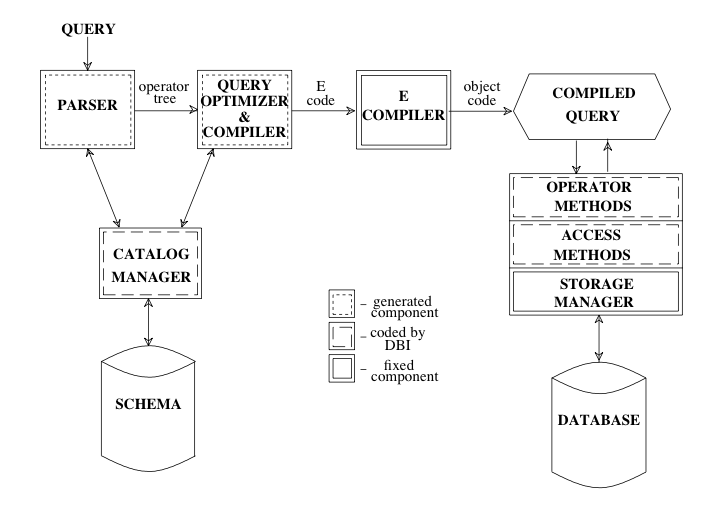
\includegraphics[width=\textwidth]{02_Grundlagen/ExodusDatabaseSystemStructure.png}
  \caption{Exodus Database System Structure}
\end{figure}

Der Baukasten von EXODUS erlaubt besteht sowohl aus Bestandteilen, die fix vorgegeben und nicht verändert werden sollen, Bausteinen die generiert werden und Teilen, die speziell entwickelt werden müssen. Der Werkzeugkasten umfasst dabei nicht nur die Bausteine, sondern auch die Werkzeuge zur Bearbeitung und Generierung. Zu den Werkzeugen gehören ein Tool zur Erstellung eines Front-Ends für die Anfragesprache, ein Query Optimizer Generator und die Programmiersprache E (zusammen mit einem passenden Compiler). Mit Hilfe des Tools zur Erstellung eines Front-Ends für Anfragesprachen kann die Parser Komponente generiert werden. Der Query Optimizer wird als Resultat des Query Optimizer Generators erzeugt. (vgl. Fig. Exodus Database System Structure)

Neben den generierten Komponenten gibt es den E Compiler, der E Code in Objekt-Code übersetzt. Er kommt zum Einsatz, um die durch den Query Optimizer optimierte Anfrage in eine kompilierte Anfrage umzusetzen. Diese Komponente ist ähnlich wie der Storage Manager, der für die Verwaltung von Daten in der Datenbank genutzt wird unveränderlich. 

Zwischen der kompilierten Anfrage und dem Storage Manager kommen zwei Komponenten zum Einsatz, die von einem DBI geschrieben werden müssen: Die Operator Methoden und Access Methoden. Diese beiden Komponenten dienen dazu die Anfrage in Code zu übersetzen, der durch den  Storage Manager ausgeführt wird.

Bei der Implementierung eines Optimierer kommen grundsätzlich zwei mögliche Ansätze in Frage: (1) interpretierte und (2) kompilierte Programmiersprachen. Bei EXODUS wurde zuerst die Implementierung mittels sog. "AI" Sprachen versucht. In einem Prototypen wurde mit Hilfe von Prolog ein Optimierer entwickelt. Für Prolog wurde sich entschieden, da diese Sprache Pattern Matching und eine Search Engine bereitstellt. (Auch unification konnte zum Einsatz gebracht werden, um elegant Query Trees zu erstellen.) Der Hauptvorteil eines interpretierten Ansatzes war aus Sicht von EXODUS die Möglichkeit neue Regeln zur Laufzeit des Programms hinzuzufügen. Trotz dieser Vorteile wurde der Ansatz als zu langsam verworfen. Auch der Vorteil Regeln während der Laufzeit hinzuzufügen, wird in der Literatur (QUELLE) als wenig nützlich bewertet. Statt dieses Ansatzes wurde in der Folge auf die Erstellung eines Generators, der in C geschrieben wurde, gesetzt. Der Generator erstellt basierend auf Regeln einen Optimierer in C, der wiederum kompiliert werden kann. Zwar war die Entwicklung des C Generators aufwendiger als die Implementierung in Prolog, jedoch konnte auf applikationsspezifische Notwendigkeiten, wie die Implementierung von speziellen Suchverfahren, Punkt genau eingegangen werden.


Der generierte Optimierer funktioniert so, dass er den Anfragenbaum Schritt für Schritt transformiert. Die Information über bereits erstellte Baum-Alternativen wird in einer Datenstruktur namens MESH gespeichert. MESH wird auserdem genutzt um plänge für Anfragenbäume zu speichern, die nicht beschnitten werden von der Daten Struktur. Zu jedem Zeitpunkt während der Optimiererung kann eine grosse Menge an weiteren möglichen Transformationen. Diese wird in der Datenstruktur "OPEN" gespeichert. Sie ist eine Priority Queue. OPEN ist initalizisiert mit Transformationen, die auf den initalen Tree angewendet werden können. Grundsätzlich funktioniert der Algorithmus wie folgt:

\begin{lstlisting}[caption={Exekution in EXODUS}]
While (OPEN is not empty)
	SELECT a transformation from OPEN
	Apply it to the correct node(s) in MESH
	DO method selection and cost analysis for the new nodes
	Add newly enabled transformations to OPEN

\end{lstlisting}

\subsubsection{Volcano}

Volcano ist der verbesserte Nachfolger von Exodus. Zuerst war Volcano nur ein erweiterbares, paralleles System zur Anfragenausführung. Später wurde ein neuer Anfragenoptimierer-Generator hinzugefügt. 

Der Volcano-Optimizer-Generator wurde designt und implementiert 





\subsubsection{Volcano Optimizer Generator}

Der Volcano Optimizer unterscheidet sich verglichen zu seinem Vorgänger EXODUS durch höhere Erweiterbarkeit. Er bietet Unterstützung für nicht triviale Kostenmodelle und physische Eigenschaften wie die Sortierreihenfolge von Relationen. Ausserdem ist er effizienter durch die Kombination von dynamischer Programmierung, zielgerichteter Suche und “Branch-and-Bound-pruning.” Im Vergleich zu anderen regelbasierten Optimieren ist das System unabhängig von einem gegebenen Datenmodell.

\subsubsection{Volcano Optimizer Generator}

Bei der Generierung eines Plans auf Grund einer Anfrage kommt bei Volcano ein Optimierer zur Anwendung, der speziell für den Anwendungsfall generiert wurde. Der Optimierter ist das Resultat einer Model Spezifikation, die von einem Datenbank Implementierer (DBI) erstellt und durch einen Optimierer Generator in Source Code umgewandelt wird. Dieser Code wird mit Hilfe eines Compilers in das Endprodukt, den Optimierer, umgewandelt.

 \subsubsection{Design Prinzipien}

Der Optimierer folgt dabei fünf Designentscheidungen \cite{graefe1993volcano}, die die Erweiterbarkeit und eine Effiziente Suche des Optimiers erlauben.

\begin{itemize}

\item Die erste Grundlage des Volcano Optimizers ist die Anwendung von algebraischen Techniken wie algebraische Operatoren und Äquivalenzklassen. Volcano unterscheidet dabei zwischen logischer und phypsicher Algebra. Die Umwandung von logischer Algebra (der Anfrage) in die physische Algebra (einem Query Evaluation Plans) gescheit bei durch die Transformation der logischen Algebra mit Hilfe von Kostenbasierten Mappings von Logischen Algorithmen.


\item Das zweite Prinzip sieht vor, dass die Information über algebraische Gesetze, die zur Transformation von Algebraischen Ausdrücken genutzt werden als Regeln und Pattern modular erfasst sind. Durch dieses prinzip sind die einzelnen Regeln klar und transparent von einander getrennt und können zu Regelsets zusammengestellt werden. Einige dieser Regelsets werden im folgenden Kapitel behandelt.


\item Das dritte Prinzip betrifft den Input des Optimierers im Gegensatz zu anderen Optimieren (namentlich Stardust) setzt der Volcano Optimizer auf algebraische Äquivalenzen als Input Parameter. Andere System nutzen hier mehrere Stufen an Umwandlung, um zwischen Query und Optimizer Input zu vermitteln. 

\item Kompilierung über Interpretierung von Regeln ist das vierte Prinzip, das zur Anwendung kommt. Da es sich bei der Generierung von äquivalenten Plänen um ein CPU intensives Geschäft handelt, wurde entscheiden, dass die Regeln zur Transformation der Pläne kompiliert und nicht interpretiert werden. Zwar verliert der Optimierer daduch die Möglichkeit ad hoc neue Regeln in den Optimierer aufzunehemen. Diese Möglichkeit wird jedoch in der Praxis nicht benötigt.

\item Das letzte Prinzip ist, dass der Volcano Optimierer auf dynamisches Programmieren bei der Generierung von Programmen setzt. 


\end{itemize}





